%%%%%%%%%%%%%%%%%%%%% RJT TeX Template %%%%%%%%%%%%%%%%%%%%%
\documentclass[twoside,11pt,a4paper]{article}

%%%% BHAM PREAMBLE - SET THIS FIRST! %%%%
\newcommand{\bhamstudentname}{Sarathkumar Padinjare Marath Sankaranarayanan}
\newcommand{\bhamthesistitle}{Machine Learning \& Deep Learning Approaches to Predict Credit Card Default}
\newcommand{\bhamfronttitle}{Machine Learning \& Deep Learning Approaches \\ to Predict Credit Card Default}
\newcommand{\bhamschool}{School of Computer Science}
\newcommand{\bhamcollege}{Engineering and Physical Sciences}
\newcommand{\bhamdegree}{MSc. Artificial Intelligence \& Computer Science}
\newcommand{\bhamid}{2359859}
\newcommand{\bhamsupervisor}{Dr.Kashif Rajpoot}
\newcommand{\bhamyear}{2022}
%%%%           %%%%


\usepackage[hyphens]{url}
\usepackage[breaklinks]{hyperref}
\usepackage{fancyhdr}
\usepackage[sort]{natbib} 
\usepackage{comment} % from http://www.latex-community.org/forum/viewtopic.php?f=5&t=4538
\usepackage{dirtree} % from http://blog.plenz.com/2011-07/represent-directory-structures-in-latex.html
\usepackage{longtable} % from http://stackoverflow.com/questions/2896833/how-to-stretch-a-table-over-multiple-pages
\usepackage{algorithm}   
\usepackage{algorithmic}   %both algorithm* from http://hasini-gunasinghe.blogspot.co.uk/2014/02/presenting-algorithmsprotocols-in-neat.html

\renewcommand{\algorithmiccomment}[1]{#1} %http://tex.stackexchange.com/q1uestions/61861/algorithmic-package-for-loop-and-comment-at-the-same-line
\usepackage[printonlyused]{acronym}

\pagestyle{fancy}
\renewcommand{\sectionmark}[1]{\markboth{#1}{}}	%from tex.stackexchange.com/questions/111361

\lfoot{\bhamstudentname}
\cfoot{}
\rfoot{}
\fancyhfoffset[L]{0cm} %this fixes the right page number margin issue.
\newcommand{\HRule}{\rule{\linewidth}{0.5mm}}
\renewcommand{\headrulewidth}{0pt}
\newcommand{\tab}{\hspace*{1.25em}}
\newcommand{\minitab}{\hspace*{0.25em}}

%footnote stuff
\usepackage{perpage}
\MakePerPage{footnote} %the perpage package command
\renewcommand*{\thefootnote}{\fnsymbol{footnote}}

\lhead{}\chead{}\rhead{}
\setlength{\headheight}{28pt} %fixes the warnings about headheight being too small
\setlength{\headsep}{6pt}
\pdfoutput=1 % we are running PDFLaTeX
\usepackage[left=2.55cm,right=1.6cm,top=1.8cm,bottom=1.8cm]{geometry}
\usepackage{titling}	
\setlength{\droptitle}{-2.75cm}   % This is your set screw\\
\usepackage{titlesec}
\titleformat*{\section}{\normalsize	\bfseries}
\titleformat*{\subsection}{\small \bfseries}
\titleformat*{\subsubsection}{\footnotesize \bfseries}
%modifies the size of the gaps between the top of the title and bottom
% arguments {type}{left}{top}{bottom}
\titlespacing*{\section} {0pt}{3ex plus 1ex minus .2ex}{2ex plus .2ex}
\titlespacing*{\subsection} {0pt}{2.25ex plus 1ex minus .2ex}{0.75ex plus .2ex}
\titlespacing*{\subsubsection}{0pt}{2.ex plus 1ex minus .2ex}{0.5ex plus .2ex}

\setlength{\intextsep}{0pt} %from http://tex.stackexchange.com/questions/25828/how-to-remove-change-the-vertical-spacing-before-and-after-an-algorithm-environ

\usepackage[pdftex]{graphicx}
\graphicspath{ {figures/} }

\usepackage{enumitem}
\usepackage{pdfpages}
\usepackage{lastpage}
\usepackage{amsmath}
\usepackage{amsfonts}
\usepackage{amssymb}


\usepackage{epstopdf} %http://dirkraffel.com/2007/11/19/include-eps-files-in-latex/comment-page-2/

\usepackage{listings}
\lstset{
 basicstyle=\ttfamily,
  columns=fullflexible,
  keepspaces=true,
breaklines=true
} %from http://tex.stackexchange.com/questions/121601/automatically-wrap-the-text-in-verbatim

\newcommand{\todo}[1]{\textcolor{red}{TODO: #1}\PackageWarning{TODO:}{TODO found: #1!}} %from http://tex.stackexchange.com/questions/9796/how-to-add-todo-notes

\DeclareGraphicsExtensions{.jpg,.png}
%%%%%%%%%%%%%%%%%%%%%  END of TEMPLATE %%%%%%%%%%%%%%%%%%%%%

\title{MSc. Project\\\bhamthesistitle}
\author{\textsf{\bhamstudentname {\textsf{}}}}

\date{}
\begin{document}

\pagenumbering{gobble} % fix at	 http://tex.stackexchange.com/questions/7355/how-to-suppress-page-number
% this came from http://en.wikibooks.org/wiki/LaTeX/Title_Creation and http://tex.stackexchange.com/questions/14778/error-with-hrule
\begin{titlepage}
\begin{center}
% this was from http://tex.stackexchange.com/questions/7219/how-to-vertically-center-two-images-next-to-each-other
\begin{minipage}{6in}
  \centering
  \raisebox{-0.5\height}{
\includegraphics[width=1.25in]{crest}}
  \hspace*{.2in}
  \raisebox{-0.5\height}{
\includegraphics[height=0.9375in]{uni}}
  \end{minipage}
  \\ [1.0cm]
\textsc{{\LARGE \bhamschool\\}College of \bhamcollege}\\[3.5cm]

\textsc{\Large MSc. Project}\\[0.5cm]

% Title
\HRule \\[0.4cm]
\begin{center}\Huge
\bhamfronttitle
\end{center}
\HRule \\[1.5cm]
% Team and Members

\begin{center}
Submitted in conformity with the requirements\\ for the degree of \bhamdegree\\
\bhamschool\\ University of Birmingham\\
\vspace{2cm}
\bhamstudentname \\
Student ID: \bhamid\\
Supervisor: \bhamsupervisor      
\end{center}
\vfill

% Bottom of the page
{\large September \bhamyear}

\end{center}
\end{titlepage}

\section*{\centering Abstract}	


% Taken from the MSc Thesis template, and edited for a PGT report
The material contained within this report has not previously been
submitted for a degree at the University of Birmingham or any other university.
The research reported within this report has been conducted by the author
unless indicated otherwise.\\
\\
\textbf{Keywords} Credit Card Default Prediction, Ensemble Learning

\vfill
\clearpage

\section*{\centering Declaration}
% Taken from the MSc Thesis template, and edited for a PGT report
The material contained within this report has not previously been
submitted for a degree at the University of Birmingham or any other university.
The research reported within this report has been conducted by the author
unless indicated otherwise.\\
\\
\textbf{Signed} Sarathkumar Padinjare Marath Sankaranarayanan 

\vfill
\clearpage
\begin{center}
\vspace*{\fill}
\begin{minipage}{6in}

%\centering \Large{``Most men who have really lived have had, in some share, their great adventure.\\This railway is mine."}\\{\normalsize{\textsc{James J. Hill}}, \emph{Railway Pioneer}} \vspace{2cm}

%\centering \Large{``Steam engines don't answer back.\\ You can belt them with a hammer and they say nowt."}\\{\normalsize{\textsc{Fred Dibnah}}, \emph{Steeplejack and Engineer}} \vspace{2cm}

\centering \Large{``You have to learn the rules of the game.\\ And then you have to play better than anyone else"}\\{\normalsize{\textsc{Albert Einstein}}}

  \end{minipage}
  \vspace*{\fill}
\end{center}


\clearpage
\maketitle
\vspace{-5.5em} %fixes distance between \maketitle and the TOC
\begingroup
    \fontsize{9pt}{11pt}\selectfont
\tableofcontents
\endgroup
\clearpage
\phantomsection
\section*{Table of Abbreviations}

\normalsize
\begin{acronym}[SCEPTICS] % Give the longest label here so that the list is nicely aligned
\acro{SVM} {Support Vector Machine}
\acro{ANN} {Artificial Neural Network}
\acro{GBDT} {Gradient Boosting Decision Tree}
\acro{GRU} {Gated Recurrent Unit}
\acro{LGBM} {Light Gradient Boosting Machine}
\acro{XGBoost} {Xtreme Gradient Boosting Machine}
\acro{GRU} {Gated Recurrent Unit}
\acro{CV}{Cross Validation}
\acro{SMOTE}{Synthetic Minority Oversampling Technique}
\acro{RAM}{Random Access Memory}
\acro{MSE}{Mean Squared Error}
\acro{ReLU}{Rectified Linear Unit}
\acro{CFS}{Correlation Based Feature Selection}
\acro{AUC}{Area Under the Curve}
\acro{PCA}{Principle Component Analsys}
\acro{RNN}{Recurrent Neural Network}
\acro{RF}{Random Forest Classifier}
\acro{KNN}{K-Nearest Neighbours}
\acro{RBF}{Radial Basis Function}
\acro{DT}{Decision Tree Classifiers}
\acro{GOSS}{Gradient based One-side Sampling}
\acro{TP}{True Positive}
\acro{TN}{True Negative}
\acro{FP}{False Positive}
\acro{FN}{False Negative}
\end{acronym}


\addcontentsline{toc}{section}{Table of Abbreviations} 
\clearpage


\listoffigures

\addcontentsline{toc}{section}{List of Figures} 
\clearpage

% set up the page numbering and counter - Table of Abbreviations has no page number
% also set up the footers and headers appropriately.
\pagenumbering{arabic}
\setcounter{page}{1}
\lhead{}\chead{MSc. Project Report :: \nouppercase{Section \thesection\minitab :: \leftmark}}\rhead{}
\rfoot{Page \thepage \hspace*{0.2pt} of \pageref{LastPage}}
\renewcommand{\headrulewidth}{0.4pt}

\section{Introduction}
The objective of this project was to create a machine learning model to predict credit card default on an industrial-scale dataset. 7 different machine learning models \& 3 deep learning architectures were explored during the experimentation phase. 


\subsection{Definitions}
This section introduces definitions for terms that are important for understanding the problem.

\subsubsection{Credit Card Statement Date}
The credit card statement date is the date on which the statement/bill is generated every month. Any transaction conducted on the card post billing date will reflect in the next month's credit card statement.

\subsubsection{Delinquent Account}
A credit card account is considered delinquent if the customer has failed to make the minimum monthly payment for 30 days from the original due date.

\subsubsection{Delinquency Rate}
The percentage of credit card accounts within a financial institution's portfolio whose payments are delinquent.
\begin{equation}
	Delinquency Rate = \left(\frac{Number of Delinquent Credit Card Accounts}{Total Number of Credit Card Account}\right) * 100
\end{equation}

\subsubsection{Credit Card Default}
The customer is considered as defaulting customer in the event of nonpayment of the due amount in 120 days after the latest statement date.

\subsection{Motivation}

\begin{figure}[ht]
	\centering
	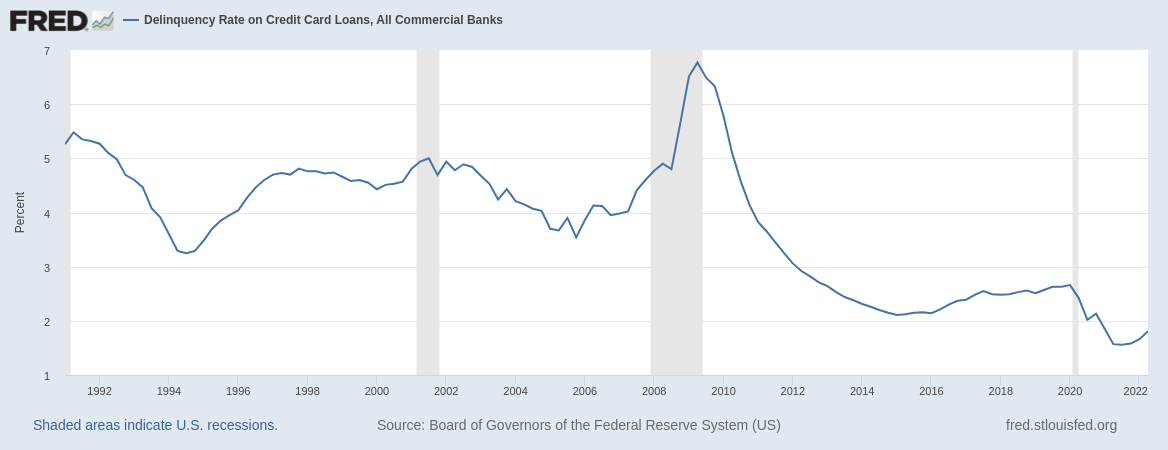
\includegraphics[width=1.0\textwidth]{fredgraph}
	\caption[]{Delinquency rate on credit card loans for the period 1992-2022\citep{fedgraph_delinquency_history}.}
\end{figure}
\subsection{Aim \& Approach}
asdfasd
\subsection{Structure of Report}
safsdfd

\vfill
\clearpage
\section{Background Knowledge}
asdfsd
\subsection{Summary}
sadfsd

\vfill
\clearpage
\section{Literature Review}
asfsf
\subsection{Summary}
dfsadfsd

\vfill
\clearpage
\section{Materials}
asdfsd
\subsection{Dataset}
asfsf
\subsection{Tools \& Software}
asfsf

\vfill
\clearpage
\section{Methodology}
asfsf
\subsection{Summary}
dfsadfsd

\vfill
\clearpage
\section{Results \& Discussions}
asfsf
\subsection{Summary}
dfsadfsd

\vfill
\clearpage
\section{Conclusion \& Summary}
asfsf
\subsection{Summary}
dfsadfsd

\vfill
\clearpage

\lhead{}\chead{MSc. Project Report :: \nouppercase{\leftmark}}\rhead{}
\phantomsection
\addcontentsline{toc}{section}{References}
\bibliographystyle{agsm} 
\bibliography{mybib}

\clearpage

\section{Appendix One: Code}

\subsection{Directory Structure}

\subsection{Running the Provided Code}

\clearpage
\end{document}
